%Literature Survey
\section{The Electric Arc}
The electric arc in a CB plays a major role in the interruption process which changes the status of breaker from conducting to a non-conducting state. An electric arc is the switching element of CB. Arc has nonlinear characteristics. The surface contact area is very small when the contacts are separated. As a result, the high current density increases the temperature that dissociates the molecules into atoms. Further increase in energy level, orbital electrons of the atoms dissociates into free moving electrons, leaving positive ions which lead to a plasma state. The Saha's equation gives the relation between the temperature T, the gas pressure P, and the fraction f of the atoms that are ionized
\begin{equation}
\frac{f^2}{1-f^2}P = 3.16 \times 10^{-7} T^{5/2} e^{-e V_i/ kT}
\end{equation}

where\\
$e ~= 1.6 \times 10^{-19}$, the charge of an electron \\
$V_i=$ ionization potential of the gaseous medium \\
$k ~= 1.38 \times 10^{−23}$, Boltzmann's constant

As shown in the figure \ref{fig:Potential Distribution Along an Arc Channel [2]}, the electric arc can be divided into three regions- the cathode region, the middle column, and the anode region. The figure also shows a potential distribution along the arc channel between the breaker contacts. The voltage drop near anode is around 5-10 volts whereas it is around 10-25 volts near the cathode region. Magnitude of arc current, length of column, types of gases and gas pressure are the parameters on which the voltage drop in the arc column depends \cite{garzon2002high}

\begin{figure}[!htbp]
    \centering
    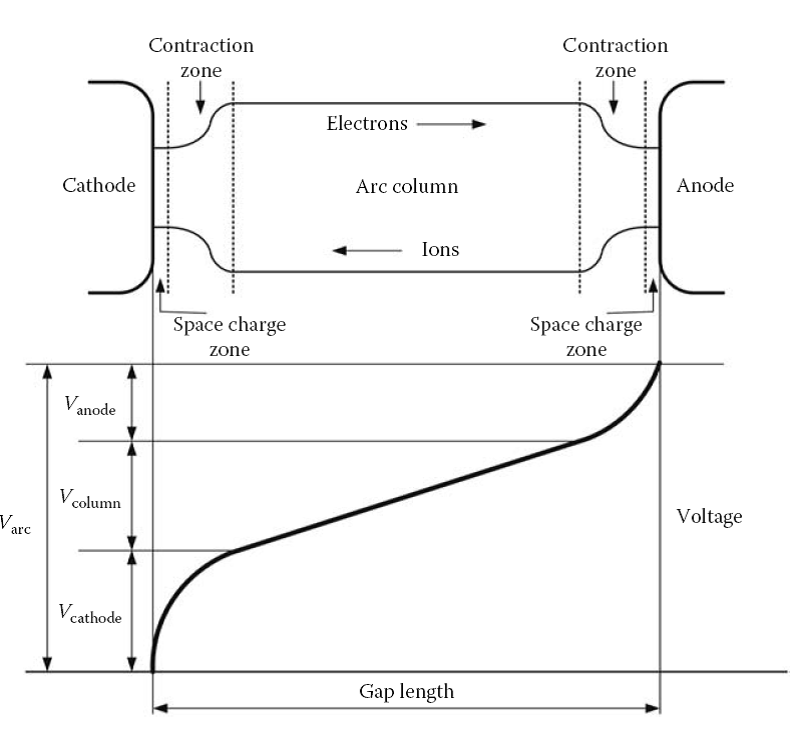
\includegraphics[width=\textwidth]{PotentialDistributionAlonganArcChannel}
    \caption[Potential Distribution Along an Arc Channel]{Potential Distribution Along an Arc Channel \cite{van2001transients}}
    \label{fig:Potential Distribution Along an Arc Channel [2]}
\end{figure}

\subsection[Time-intervals in the interruption process of an electric arc]{Time-intervals in the interruption process of an\\ electric arc}
CB is generally stressed in four intervals during fault current interruption:
\begin{itemize}
\item High current phase
\item Interaction interval
\item Dielectric recovery phase during TRV buildup
\item Dielectric withstand phase during TRV peak and recovery voltage
\end{itemize}
The intervals of CB stresses are shown in figure \ref{fig:Intervals and Failure Modes in the Interruption Process [24]}.

\begin{figure}[!htbp]
    \centering
    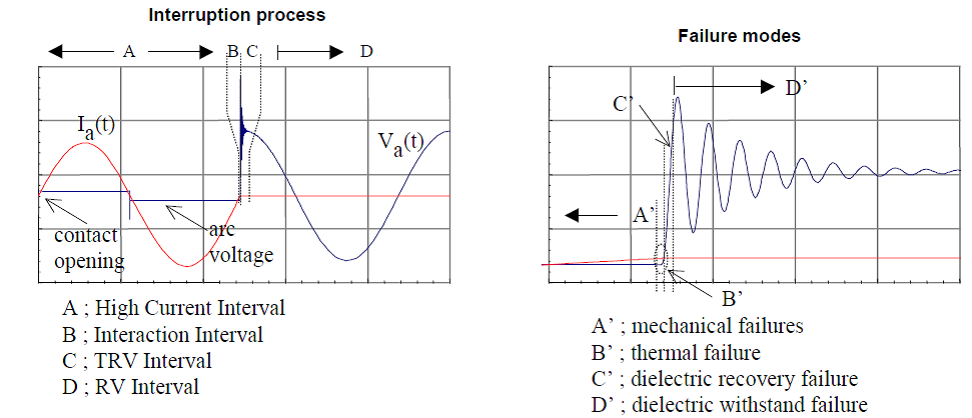
\includegraphics[width=\textwidth]{IntervalsandFailureModesintheInterruptionProcess}
    \caption[Intervals and Failure Modes in the Interruption Process]{Intervals and Failure Modes in the Interruption Process \cite{browne1984circuit}}
    \label{fig:Intervals and Failure Modes in the Interruption Process [24]}
\end{figure}

Every interval during interruption stage has specific characteristics:
\begin{itemize}
\item high volume energy input during high current phase in the arc may cause the CB to overheat or result in mechanical damage
\item possibility of reignition in interaction interval during thermal stress in arc circuit interaction
\item dielectric stress which may cause a dielectric failure of the gap between the breaker contacts during the dielectric recovery and dielectric withstand period
\end{itemize}

\section{Arc-Circuit Interaction}
Interaction of several phenomena makes the current interruption process in a high-voltage circuit breaker a complex matter. At current zero arc diameter decreases with~ the cross section~ approximately~ proportional~ to the current. ~Current interruption of the CB occurs normally at current zero. During the current interruption process strong interaction exists between the physical process between the breaker contacts and the connected network.

Figure \ref{fig:Representation of the Network Connected to the Breaker Terminals} shows the representation of the network connected to the breaker terminals.\\

\begin{figure}[!htbp]
    \centering
    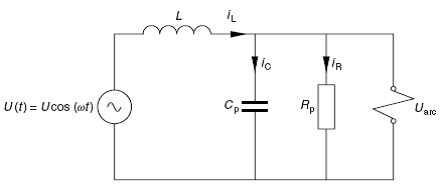
\includegraphics[width=\textwidth]{RepresentationoftheNetworkConnectedtotheBreakerTerminals}
    \caption[Representation of the Network Connected to the Breaker Terminals]{Representation of the Network Connected to the Breaker Terminals \\ \medskip \footnotesize{$L$ - Total series inductance of the network; $C_p$ - Total stray capacitance; $R_p$ - Characteristic impedance of the connected overhead lines}}
    \label{fig:Representation of the Network Connected to the Breaker Terminals}
\end{figure}

During current interruption two physical requirements are involved:
\begin{itemize}
\item Thermal regime: The hot arc channel in the arcing region has to be cooled down so that the medium stops conducting
\item Dielectric regime: The recovery voltage after the arc extinction contains high frequency transient component, Transient Recovery Voltage, which rapidly increases. The dielectric medium between the contacts must withstand this TRV for successful interruption
\end{itemize}

The current will flow for another half cycle till the next current zero if any of the above requirement is not met. Figure \ref{fig:Curves of Short Circuit Current and Recovery Voltage} shows the curves of short circuit current and recovery voltage and stresses on the extinction chamber at interruption.

\begin{figure}[!htbp]
\centering
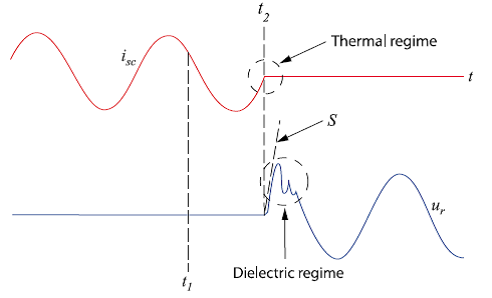
\includegraphics[width=\textwidth]{CurvesofShortCircuitCurrentandRecoveryVoltage}
\caption[Curves of Short Circuit Current and Recovery Voltage]{Curves of Short Circuit Current and Recovery Voltage \cite{Livetankcircuitbreaker}\\\medskip \footnotesize{$t_1$ - contact separation; $t_2$ - arc extinction; $S$ - rate of rise of recovery voltage}}
\label{fig:Curves of Short Circuit Current and Recovery Voltage}
\end{figure}

\subsection{Thermal regime}
\setlength{\parskip}{1em}
 The thermal regime between the CB contacts during arc interruption depends upon the initial rate of rise of the transient recovery voltage (du/dt) immediately after current zero and the rate of decrease of the current to be interrupted (di/dt). Higher values of either of these two parameters make the interruption more severe. A high value of di/dt makes the interruption difficult due to a large amount of stored energy at current zero.  High values of du/dt will result in an increase of the energy to the post-arc current. Post arc current up to few amperes flows after current zero due to electrical conductivity left in the arc path as shown in figure \ref{fig:Current Shapes at Interruption}. The successful interruption depends on the race between the energy input in the arc path by the TRV and the cooling effect.

The thermal breakdown of CB will occur if the energy input is more.

\setlength{\parskip}{0em}
\begin{figure}[!htbp]
\centering
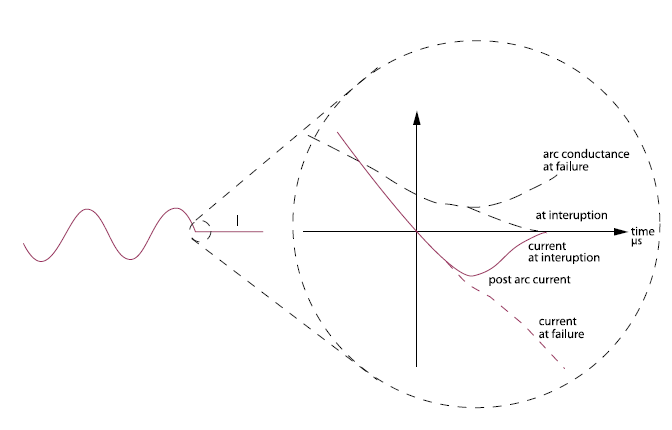
\includegraphics[width=\textwidth]{CurrentShapesatInterruption}
\caption[Current Shapes at Interruption]{Current Shapes at Interruption \cite{Livetankcircuitbreaker}}
\label{fig:Current Shapes at Interruption}
\end{figure}

\subsection{Dielectric regime}
In the dielectric regime, the temperature of the extinguishing medium is much higher than the ambient who reduce the voltage withstand capability of the contact gap. The stress on the CB depends on the Rate of Rise of Transient Recovery Voltage (RRRV). The interruption is successful if the rate of recovery of the contact gap at the instant of current zero is higher than RRRV otherwise dielectric failure will occur. Figure \ref{fig:Dielectric Interruption Regime} shows the successful and failure interruption in dielectric interruption regime.

\begin{figure}[!htbp]
\centering
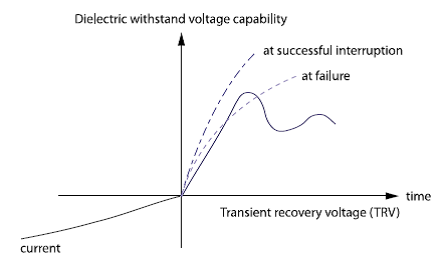
\includegraphics[width=\textwidth]{DielectricInterruptionRegime}
\caption{Dielectric Interruption Regime}
\label{fig:Dielectric Interruption Regime}
\end{figure}

\section{Circuit Breaker Modeling during Opening Operations}
CB models are needed to analyze both closing and opening operations. The separation of the contacts of the CB causes the formation of an electric arc. The main objectives of a circuit breaker model are \cite{EPRIReportEL4651}:

\begin{itemize}
\item to determine all voltages and  currents that are produced in the system due to switching action of breaker
\item to determine the reliability of CB operation under given set of conditions for the system
\end{itemize}

Modeling guidelines for CBs during closing and opening operations proposed by CIGRE WG 33-02 are shown in Table \ref{table:Modeling Guidelines for Circuit Breakers}

\begin{table}[!htbp]
\begin{threeparttable}
\renewcommand{\arraystretch}{0.9}
\caption[Modeling Guidelines for Circuit Breakers]{Modeling Guidelines for Circuit Breakers \cite{cigre199033}}
\label{table:Modeling Guidelines for Circuit Breakers}
\centering
\small
\begin{tabular}{| >{\centering\arraybackslash}m{0.5in} | >{\centering\arraybackslash}m{0.9in} | >{\centering\arraybackslash}m{0.91in} |>{\centering\arraybackslash}m{0.91in} | >{\centering\arraybackslash}m{0.91in} | >{\centering\arraybackslash}m{0.75in} |}
\hline
\multicolumn{2}{|c|}{\textbf{Operation}} & \textbf{Low-Frequency Transients} & \textbf{Slow Front Transients} & \textbf{Fast Front Transients}	&	\textbf{Very Fast Front Transients} \\ \hline
\multirow{2}{*}{Closing}& Mechanical pole spread & Important & Very important & Negligible & Negligible \\ \cline{2-6}
				 		& Prestrikes & Negligible & Important & Important & Very important \\ \hline
				 		
\multirow{4}{*}{Opening}& High current interruption & Important for interruption capability studies only & Important for interruption capability studies only & Negligible & Negligible \\ \cline{2-6}
						& Current chopping & Negligible & Important for interruption capability studies only & Important for interruption capability studies only & Negligible \\ \cline{2-6}
						& Restrike characteristics & Negligible & Important for interruption capability studies only & Very important & Very important \\ \cline{2-6}
				 		& High-frequency current interruption & Negligible & Important for interruption capability studies only &	Very important & Very important \\ \hline
\end{tabular}
\end{threeparttable}
\end{table}

\section{Arc Modeling}
\setlength{\parskip}{1em}
The design of interrupting chamber of HVCBs plays an important role in the arc interruption. Arc models were used for the better understanding of current interruption process. However, the physical phenomena involved in the current interruption is very complex. Hence it is not possible to use the arc models for CB design. However, arc models can be used for arc circuit interaction. Arc models are able to simulate the nonlinear behavior of the CB arc. Correct numerical treatment of the arc circuit problem is important due to nonlinear behavior of the arc and small time constants.

To reproduce the arc interruption phenomenon in the testing, operation, and development of CBs several approaches can be used \cite{anke1988practical}. Arc models can be classified into three categories \cite{van2001transients}.

\setlength{\parskip}{0em}
\begin{itemize}
\item Physical arc models
\item Parameter models
\item Black box arc models ( P-$\tau$ models)
\end{itemize}

\subsection{Physical arc models (PAM)}
In physical arc models, the physical process is considered in detail. The behavior of the arc is calculated from conservation laws, gas and plasma properties, and exchange mechanisms (radiation, heat conduction, turbulence). The design engineers use physical arc models for designing a new prototype. Equations \ref{eq:2.2} to \ref{eq:2.4} describe the physical arc model.

Conservation of mass:
\begin{equation} \label{eq:2.2}
\frac{\partial \rho}{\partial t} + div(\rho u) = 0
\end{equation}

Conservation of momentum:
\begin{equation} \label{eq:2.3}
\rho \frac{\partial u}{\partial t} + \rho(u \cdot grad)u = -grad(p)
\end{equation}

Conservation of energy:
\begin{equation} \label{eq:2.4}
\underbrace{\rho \frac{\partial b}{\partial t}}_{\substack{\text{change} \\ \text{of energy}\\ \text{in unit}\\ \text{volume}}}
+ 
\underbrace{u \cdot grad(\rho b)}_{\substack{\text{energy} \\ \text{input by}\\ \text{mass flow}\\ \text{convection}}}
-
\underbrace{\sigma E^2}_{\substack{\text{Joule} \\ \text{heating}}}
=
\underbrace{div(\rho u)}_{\substack{\text{work} \\ \text{performed}\\ \text{by flow}}}
+
\underbrace{div[K \cdot grad(T)]}_{\substack{\text{thermal} \\ \text{conduction}\\ \text{loss}}}
-
\underbrace{R[T, \rho]}_{\substack{\text{radiation} \\ \text{loss}}}
\end{equation}

\begin{tabular}{ >{\arraybackslash}m{3in} >{\arraybackslash}m{2.5in}}
$p$ - pressure 		 			& $\sigma$ - electrical conductivity\\
$\rho$ - gas density 			& $K$ - thermal conductivity\\
$u$ - gas flow velocity 		& $T$ - gas temperature\\
$h$ - enthalpy of gas 			& $R$ - radiation loss\\
$E$ - electric field strength	& $r$ - arc radius\\
\end{tabular}

\subsection{Black box models (BBM)}
In black box models, the arc is described by a simple mathematical equation and gives the relation between the arc conductance, arc voltage, and arc current. For arc circuit interaction in network studies, the black box models are very useful for simulation. They are based on physical considerations. The electrical behavior of the arc is important than the internal processes. In transient programs, black box models are most suitable representations \cite{anke1988practical, cigre199313}.

The aim of a black box model is to describe the interaction of the switching device and the corresponding electrical circuit during an interruption process. The aim of the Black box models is to obtain quantitatively correct performance of the CB \cite{EPRIReportEL4651}:
\begin{itemize}
\item In the simplest model the breaker is represented as an ideal switch that opens at first current-zero crossing after the tripping signal is given. This model can be used to obtain the voltage across the breaker which can be compared with a pre-specified TRV withstand capability for the breaker. This model cannot reproduce any interaction between the arc and the system

\item Arc as a time-varying resistance or conductance is used in the elaborated model. Knowledge of the initial interrupting current and breaker characteristics is used to determine the time variation. This model requires advanced knowledge of the effect of the system on the arc however the model can represent the effect of the arc on the system. Precomputed TRV curves are required to determine the adequacy of the breaker

\item  In advanced model breaker is represented as a dynamically varying resistance or conductance. The value of conductance depends on the past history of arc voltage and current. Precomputed TRV curves are not required. Generally, these models are developed to determine initial arc quenching. Some advanced models are used in determining the arc reignition in CB which occurs due to insufficient dielectric withstand capability between the breaker contacts. The effect of the arc on the system and vice versa is possible in this model
\end{itemize}

Models for representation of SF\textsubscript{6} CBs during thermal and dielectric periods were discussed and used \cite{van1992physical, van1992comparison}. Models proposed in last decades are available \cite{martinez2005parameter, avdonin1980some, maximov2009method, st1988new, schavemaker2000improved, nitu2008comparison, knobloch2001behaviour, smeets2002performance, thomas1995simulation, schavemaker1999comparison, iturregi2012considerations, karetta1998simulation, bui1997performance, liao2010study, zhang2009modelling, ziani2010application}.

\subsubsection{Cassie model}
A. M. Cassie assumed that the shape of the arc channel is a cylinder filled with an ionized gas with a constant temperature T, but with a variable diameter. It is the convection losses that govern the high current arc during the high current time interval. As the current changes, the cross section of the arc changes but the temperature inside the arc column remains constant \cite{martinez2005parameter}. For the high current region, data collected from experimental results is in good agreement with the model. However, around the current zero region, agreement is good only for high rates of current decay. Theoretically and practically, at current zero the arc diameter never decays to zero to result in arc interruption. At current zero there is a small filament of an arc remaining with a diameter of only a fraction of a millimeter. This filament is still high temperature plasma that can be easily transformed into an arc by the reappearance of a sufficiently high supply voltage. The Cassie model, in many cases, is referred to as the high current region model of an arc. This model has proved to be a valuable tool for describing the current interruption phenomena, especially when it is used in conjunction with the Mayr model.

The Cassie model is well suited for studying the behavior of the arc conductance in the high-current time interval when the plasma temperature is 8000\textdegree K or more. The Cassie model is given by equation \ref{eq:2.5}.

\begin{equation}\label{eq:2.5}
\frac{1}{g} \frac{dg_c}{dt} = \frac{1}{\tau_c} \left[\left(\frac{v}{v_0}\right)^2 - 1\right] = \frac{1}{\tau_c} \left[\left(\frac{i}{v_0g_c}\right)^2 - 1\right]
\end{equation}

\subsubsection{Mayr model}
Mayr assumed that the power losses are caused by thermal conduction at small currents, which means that the conductance is strongly temperature dependent but is independent of the cross section area of the arc. Mayr considered the arc channel to be cylindrical with a constant diameter. The model describes the arc conductance around current zero. The removal of energy from arc column is through thermal conduction. The Mayr model is suited for modeling of the arc in the vicinity of current zero when the temperature of the plasma is below 8000\textdegree K. The Mayr model is given by equation \ref{eq:2.6}

\begin{equation}\label{eq:2.6}
\frac{1}{g_m} \frac{dg_m}{dt} = \frac{1}{\tau_m} \left(\frac{v_i}{P_0} - 1\right) = \frac{1}{\tau_m} \left(\frac{i^2}{P_0g_m}- 1\right)
\end{equation}
In these equations\\ 
$g$ - arc conductance\\ 
$v$ - arc voltage\\
$i$ - arc current\\
$\tau$ - arc time constant\\
$P_0$ - steady-state power loss\\
$v_0$ - constant part of the arc voltage\\
$g_c$ is in the region of 1 $\mu s$ and $g_m$ is between 0.1 and 0.5 $\mu s$ for SF\textsubscript{6} CB.

\subsubsection{Browne model}
Mayr assumed that the arc temperature is generally above 6000\textdegree K and is likely to be in excess of 20000\textdegree K. The high temperatures lead to a linear increase of gas conductivity instead of exponential relationship. In order to take the consideration of high temperature and dynamic response representation, Mayr model must closely follow the Cassie's equation during current controlled regime. T. E. Browne recognized this need and in 1948 he developed a composite model using an equation similar to Cassie's to define the current controlled arc regime, and then converting it to a Mayr-like equation for the temperature controlled regime, and in the event that interruption did not occur at the intended current zero, he reverted again to the Cassie model. In 1958 Browne extended the application of his combined model to cover the analysis of thermal re-ignitions that occur during the first few microseconds following the critical, post current zero energy balance period. Starting with the Cassie and the Mayr equations, and assuming that before current zero the current is defined by the driving circuit, and that after current zero, the voltage applied across the gap is determined strictly by the arc circuit, Browne assumed that the Cassie equation was applicable to the high current region prior to current zero and also shortly after current zero following a thermal re-ignition. The Mayr equation was used as a bridge between the regions where the Cassie concept was applied. This model was a valuable tool that has practical applications. It has been used extensively in the design and evaluation of circuit breakers. Browne's model is given by equation \ref{eq:2.7}.
\begin{equation} \label{eq:2.7}
\frac{1}{g}= \frac{1}{g_c} + \frac{1}{g_m}
\end{equation}

\subsubsection{Avdonin model}
Avdonin proposed a model for air-blast and SF\textsubscript{6} breakers \cite{avdonin1980some}. The arc resistance of this model is expressed by equation \ref{eq:2.8}
\begin{equation} \label{eq:2.8}
\frac{dr_a}{dt}= \frac{r_a^{1-\alpha}}{A} - v_a r_a \frac{r_a^{1-\alpha-\beta}}{A B}
\end{equation}
which is derived from the modified Mayr equation \ref{eq:2.9}
\begin{equation} \label{eq:2.9}
\frac{dr_a}{dt} = \frac{r_a}{\tau} \left( 1 - \frac{v_a r_a}{P_0} \right)
\end{equation}

with

\begin{equation}
\tau = A r_a^\alpha ~~~~~~ P_0 = Br_a^\beta
\end{equation}
where\\
$r$ -  arc resistance\\
$v_a$ - arc voltage\\
$i_a$ - arc current\\
$\tau$ - arc time constant\\
$P_0$ - breaker cooling power\\

The thermal failure near current interruption and post-arc region conductivity studies are possible in this model.

\subsubsection{Urbanek model}
The Urbanek developed a model which can represent arc interruption and thermal as well as the dielectric failure \cite{maximov2009method}. Current chopping and reignition both are represented. The arc conductance is characterized by the equation \ref{eq:2.11}.
\begin{equation} \label{eq:2.11}
\frac{1}{g} \frac{dg}{dt} = \frac{1}{\tau} \left\lbrace \frac{v_i}{e^2 g} - 1 - \frac{P_0}{e^2 g} \left[ 1 - \left( \frac{v}{v_d} \right)^2 - 2 \frac{\tau}{v_d^2} v \frac{dv}{dt} \right] \right\rbrace
\end{equation}

where\\
$e$ - arc voltage for high currents\\
$P_0$ - minimum power to maintain the arc\\
$v_d$ - dielectric breakdown voltage for cold arc channel

\subsubsection{Kopplin model}
Kopplin model is used for simulation of thermal breakdown. This model is used to represent generator circuit breakers \cite{st1988new}. For the arc conductance it is characterized by a Mayr-type equation \ref{eq:2.12}
\begin{equation}\label{eq:2.12}
\frac{1}{g} \frac{dg}{dt} = \frac{1}{\tau} \left( \frac{v_i}{p_0} - 1 \right)
\end{equation}
with
\begin{equation}
\tau = K_I \cdot (g + 0.0005)^{0.25}
\end{equation}

\begin{equation}
P_0 = K_P \cdot (g + 0.0005)^{0.6}
\end{equation}

where $K_p$ and $K_I$ are model parameters.

Table \ref{table:Arc Model Applications [28]} gives the summary of applications of arc models used in the testing, development, and operation of CBs.

\begin{table}[!htbp]
\begin{threeparttable}
\renewcommand{\arraystretch}{1.3}
\caption[Arc Model Applications]{Arc Model Applications \cite{anke1988practical}}
\label{table:Arc Model Applications [28]}
\centering
\small
\begin{tabular}{| >{\arraybackslash}m{2.5in} | >{\centering\arraybackslash}m{1in} | >{\centering\arraybackslash}m{0.75in} |>{\centering\arraybackslash}m{0.75in} |}
\hline
\multicolumn{1}{|c|}{\textbf{Type of Problem}} & \textbf{Development} & \textbf{Testing} & \textbf{Operation} \\ \hline
Design optimization	&	PAM		&			&	-	\\ \hline
Mechanical system dimensioning of flow and pressure build up studies%
					&	PAM, PM	&	PAM, PM	&	-	\\ \hline
Dielectric recovery description	&	PAM, PM	&	PM	&	PM	\\ \hline
Influence of arc asymmetry and delayed current zeros	&	PAM, BBM, PM	&BBM, PM	&	PM	\\ \hline
Interruption of small inductive currents	&	PAM, BBM, PM	&	BBM, PM	&	BBM, PM	\\ \hline
Short-line fault with TRV	&	PAM, BBM, PM	&	BBM, PM	&	BBM, PM	\\ \hline
Design and verification of test circuits	&	PM	&	BBM	&	-	\\ \hline
\end{tabular}
\end{threeparttable}
\end{table}

\subsection{Parameter models (PM)}
Parameter models are basically black box models with more complex functions and tables which are derived from physical arc models and black box models.

\section{Circuit Breaker Modeling During Closing}
When the contacts of a breaker close and the gap between them get smaller, the breakdown will occur if the voltage across the gap exceeds its dielectric strength. Prestrike phenomenon during closing is shown in figure \ref{fig:Prestrike Phenomenon during Closing} \cite{martinez2009power}.

\begin{figure}[!htbp]
\centering
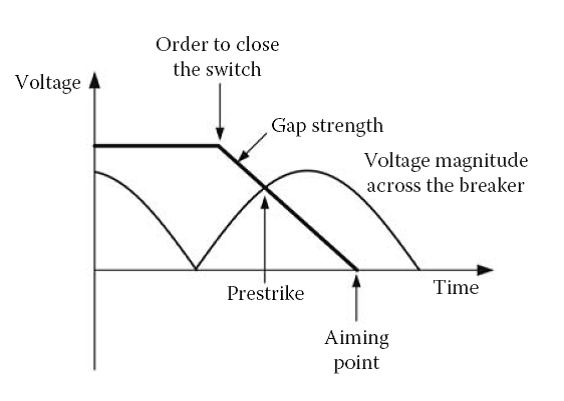
\includegraphics[width=\textwidth]{PrestrikePhenomenonduringClosing}
\caption{Prestrike Phenomenon during Closing}
\label{fig:Prestrike Phenomenon during Closing}
\end{figure}

Breaker poles closing in a multiphase breaker is random in a cycle. Hence it is difficult to determine the probability of distribution of closing time. The network on the source side or the charge trapped on transmission lines in a reclosing operation determines the peak of the transient voltages during the closing operation of CB. Instant of closing influences the maximum peak which can be different for every pole of the breaker. Many models are available to represent a CB in closing operations \cite{martinez1998digital}:
\begin{itemize}
\item In the simplest model breaker is assumed to behave as an ideal switch whose impedance changes from infinity to zero value when CB switches from open to the closing condition. The switching overvoltage across breaker depends on the closing time of breaker. For three phase system first pole to clear factor is added since all the poles do not close simultaneously. Closing instant is randomly determined in the improved approach of this model

\item In advanced approach it is assumed that there is a closing time from the instant the contacts start to close to the instant they are closed finally. Arc will strike before the contacts are completely closed if the dielectric strength of the medium is less than the withstand voltage because the withstand voltage decreases as the distance between the contacts decreases. In \cite{svensen1976influence}, pre-strike effect and its influence on the switching overvoltage during line energization is analyzed

\item  In the third approach, pre-strike dynamic arc conductance is included in the study of opening operations
\end{itemize}

\section{SF\textsubscript{6} Circuit Breakers}

\subsection{Introduction}
Figure \ref{fig:Voltage Range of Application of Breaking Technologies} shows the voltage ranges in which different breaking medium is used \cite{theoleyre1999mv}. The figure shows that SF\textsubscript{6} CBs are used in the applications for the system voltages in the range between 72.5 to 800 kV. Recently 1200 kV SF\textsubscript{6} CB is installed at Bina substation of PGCIL in Madhya Pradesh, India. Excellent dielectric strength, electron affinity or electro negativity, rapid recovery of the dielectric strength around arc region, chemically stable, non-flammable, non-corrosive, non-poisonous properties made the SF\textsubscript{6} gas superior over the other mediums used in CBs.

\begin{figure}[!htbp]
\centering
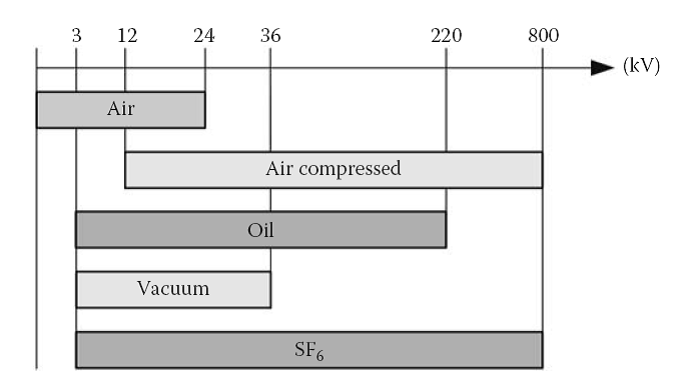
\includegraphics[width=\textwidth]{VoltageRangeofApplicationofBreakingTechnologies}
\caption{Voltage Range of Application of Breaking Technologies}
\label{fig:Voltage Range of Application of Breaking Technologies}
\end{figure}

Earlier SF\textsubscript{6} CBs were of double pressure type in which the extinguishing chamber was divided into two separate parts and were working on the principle that of air blast CBs. Nowadays puffer or self-blast principle is used for arc extinction in all high voltage SF\textsubscript{6} CBs.

\subsection{SF\textsubscript{6} puffer circuit breakers}
In the SF\textsubscript{6} puffer CBs during the opening stroke, the gas pressure for the cooling blast is created in a compression chamber. The compression of the gas will start at the same instant when the contacts start their motion during opening operation. When the arcing contacts leave the throat of the nozzle, the compressed gas is blown out along the axis of the arc. Figure \ref{fig:Main Components of the Puffer Interrupter} shows the main components of the puffer interrupter where as figure \ref{fig:Function of a Puffer Interrupter} shows its function. The current path through the closed interrupter is marked in red color.

The extinguishing pressure is current dependent in SF\textsubscript{6} puffer CBs. As seen in the no load curve figure \ref{fig:Pressure in the Puffer Cylinder at No-Load}, the maximum pressure in the puffer cylinder at no load operation is about twice the filling pressure. During a large current interruption, such as short circuit condition, gas flow through the nozzle is blocked by the arc. The arc diameter decreases during current zero which leaves more outlet area for the flow of the gas that gives maximum cooling when needed. A pressure is built up in the puffer cylinder due to blocking of the nozzle during the high current interval that may be many times the maximum no load pressure. The operating mechanism has to provide higher operating force to operate the CB due to high pressure in the puffer cylinder \cite{Livetankcircuitbreaker}.

\begin{figure}[!htbp]
\centering
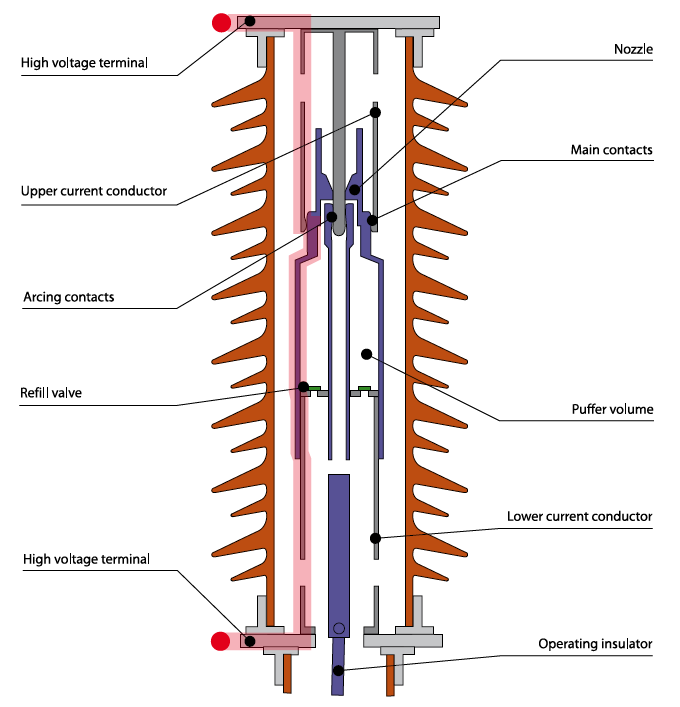
\includegraphics[width=\textwidth]{MainComponentsofthePufferInterrupter}
\caption{Main Components of the Puffer Interrupter}
\label{fig:Main Components of the Puffer Interrupter}
\end{figure}

\begin{figure}[!htbp]
\centering
\begin{minipage}{\textwidth}
\centering
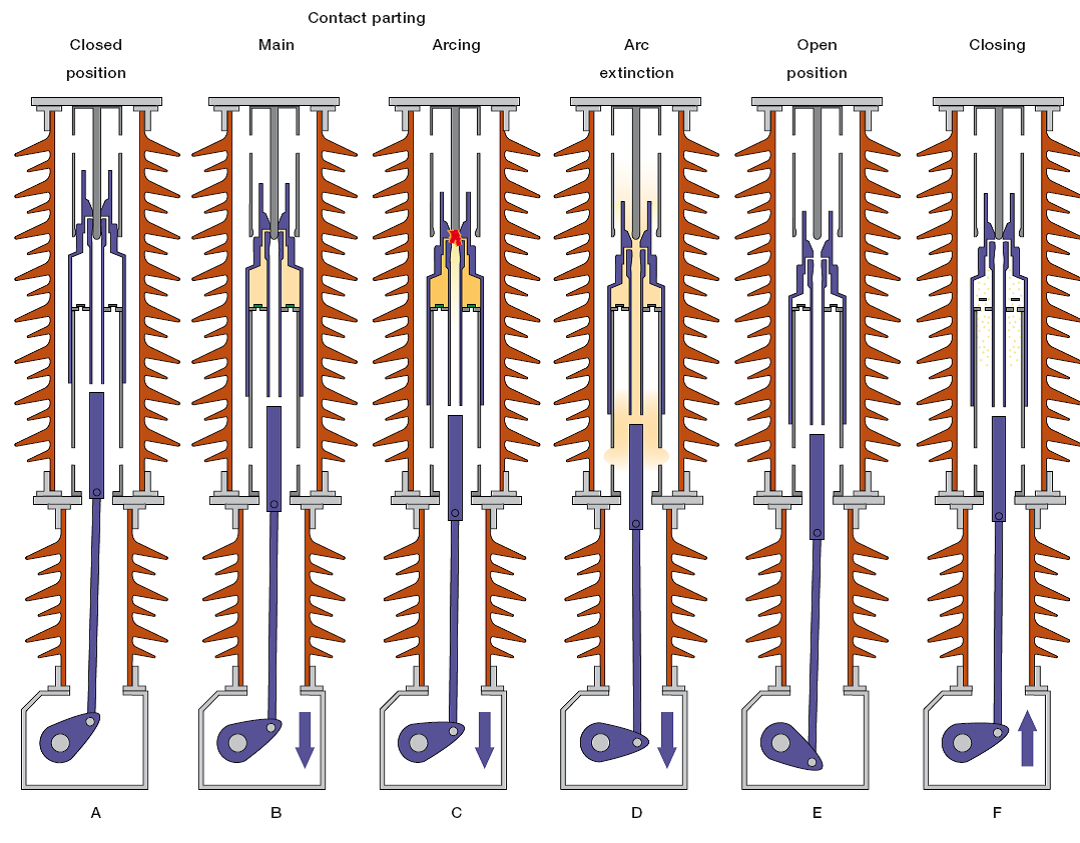
\includegraphics[width=1.1\textwidth]{FunctionofaPufferInterrupter}
\caption{Function of a Puffer Interrupter}
\label{fig:Function of a Puffer Interrupter}
\begin{flushleft}
\footnotesize A - Closed position. Current conduction through the main contacts.\\B. Main contacts separation. Starting of the moving contacts separated the main contacts commuting the current to the arcing contacts.\\C. Arc is established due to separation of arcing contacts. Pressure in the puffer cylinder starts to increase.\\
D. Arc extinction. The cold gas from the puffer volume moves rapidly through the nozzle during current zero, cooling and extinguishing the arc.\\
E. Contacts fully open.\\
F. Closing operation. Puffer volume is filled with cold gas making the interrupter ready for the next operation.
\end{flushleft}
\end{minipage}
\end{figure}

\begin{figure}[!htbp]
\centering
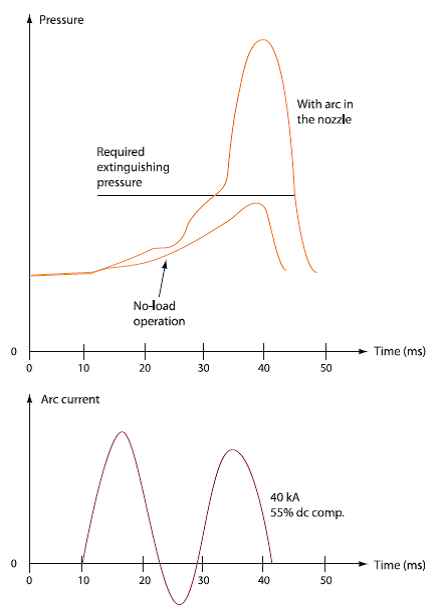
\includegraphics[width=\textwidth]{PressureinthePuffer}
\caption{Pressure in the Puffer Cylinder at No-Load and during Interruption of an Asymmetrical Short-Circuit Current of 40 kA}
\label{fig:Pressure in the Puffer Cylinder at No-Load}
\end{figure}


\subsection{SF\textsubscript{6} self-blast circuit breakers}
Most of the CB failures are of mechanical nature \cite{AlternatingCurrentCircuit}. Hence the reliability of the operating mechanism is of utmost important. In the normal puffer CB, energy from the operating mechanism is used to create the blast pressure. Self-blast principle reduced the operating energy. The arc extinction chamber in self-blast SF\textsubscript{6} CBs is divided into puffer volume and self-blast volume by the self-blast valve. During high fault current interruption, the pressure generated by the arc in the self-blast volume will be high. This high pressure closes the valve and prevents the gas from escaping into the puffer volume. The pressurized gas flows through the nozzle extinguishing the arc. But while interrupting no load current or small currents of few kA, the energy produced by the arc is insufficient to generate the pressure to close the valve. In this situation the interrupter than works as puffer interrupter.

\section{Transient Recovery Voltage}
The power system response to current interruption generates the TRV. TRV is the algebraic sum of the source side voltage and the load side voltage as shown in figure \ref{fig:Illustration of the Sources of TRV}. The shape of the TRV depends on the circuit to interrupted, characteristics of the network connections and the type of fault.

\begin{figure}[!htbp]
\centering
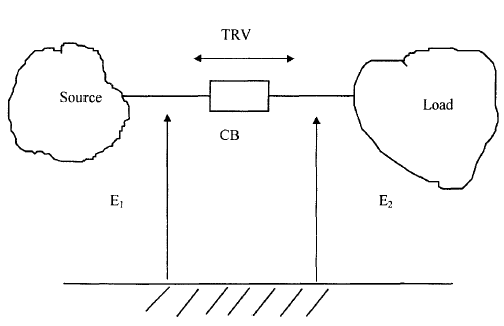
\includegraphics[width=\textwidth]{IllustrationoftheSourcesofTRV}
\caption[Illustration of the Sources of TRV]{Illustration of the Sources of TRV \cite{garzon2002high}}
\label{fig:Illustration of the Sources of TRV}
\end{figure}

IEEE and IEC both specify the standard TRV by the same approach. 
\begin{itemize}
\item The two parameters representation is used for HVCBs with a rated voltage up to 100 kV, figure \ref{fig:IEC Two and Four Parameter Limiting TRV Curves}

\item Four parameters representation is used for the CBs with rated voltage 100 kV and above, figure \ref{fig:IEC Two and Four Parameter Limiting TRV Curves}
\end{itemize}


\begin{figure}[!htbp]
\centering
\begin{minipage}{\textwidth}
\centering
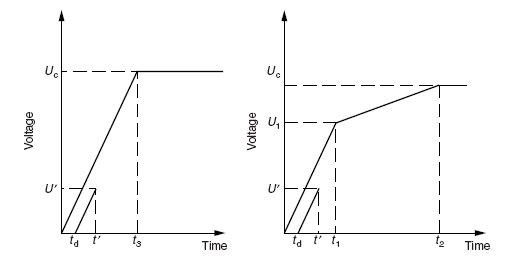
\includegraphics[width=\textwidth]{IECTwoandFourParameterLimitingTRVCurves}
\caption[IEC Two and Four Parameter Limiting TRV Curves]{IEC Two and Four Parameter Limiting TRV Curves \cite{ApplicationofTransientRecovery}}
\label{fig:IEC Two and Four Parameter Limiting TRV Curves}
\begin{flushleft}
\footnotesize \textbf{For two parameters method:}\\
$U_c$ - reference voltage, TRV peak value (kV)\\
$t_3$ - time to reach $U_c$ ($\mu s$)\\
\textbf{For four parameters method:}\\
$U_1$ - first reference voltage (kV)\\
$t_1$ - time to reach $U_1$ ($\mu s$)\\
$U_c$ - second reference voltage (TRV peak value) (kV)\\
$t_2$ - time to reach $U_c$ ($\mu s$)\\
For delay line:\\
$U^\prime$ - reference voltage (kV)\\
$t^\prime$ - time to reach $U^\prime$ ($\mu s$)\\
$t_d$ - time delay ($\mu s$)
\end{flushleft}
\end{minipage}
\end{figure}
 
The procedure and calculations necessary to apply TRV ratings for ac high-voltage circuit breakers rated above 1000 V are demonstrated in the IEEE Standard C37.011-2011 \cite{ApplicationofTransientRecovery}.

\subsection{Reactive equipment switching duty}
Switching of reactive equipment such as capacitor bank and shunt reactor is supposed to be a severe duty for CB that causes a high rate of rise of TRV across the CB contacts \cite{GuideforShuntReactorSwitching}. The high percentage of failure of CB is recorded for reactor switching and capacitor switching \cite{janssen2014international}. The inrush current during switching of isolated capacitor bank as well as back to back capacitor switching is recognized in the standards \cite{GuideforCapacitanceCurrentSwitching}. Investigations and field experience of the failure of SF\textsubscript{6} CB in the switching of 420 kV shunt reactor is presented \cite{bachiller1994operation}.  The switching transient of the shunt reactor is a high frequency response which is influenced by the surrounding circuit conditions. Figure \ref{fig:Shunt Reactor Equivalent Circuit} shows the shunt reactor equivalent circuit.

\begin{figure}[!htbp]
\centering
\begin{minipage}{\textwidth}
\centering
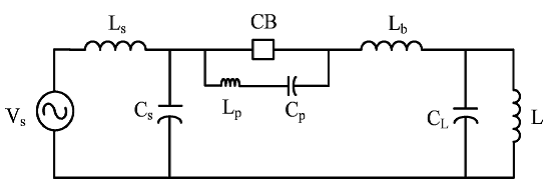
\includegraphics[width=\textwidth]{ShuntReactorEquivalentCircuit}
\caption{Shunt Reactor Equivalent Circuit}
\label{fig:Shunt Reactor Equivalent Circuit}
\begin{flushleft}
\footnotesize $L_s$ - source side inductance; $C_s$ - source side capacitance; $L_p$ and $C_p$ - stray inductance and capacitance between CB contacts; $L_b$ - the connecting series inductance; $C_L$ - load side capacitance; $L$ - shunt reactor inductance
\end{flushleft}
\end{minipage}
\end{figure}

The CB is stressed by TRV after current interruption. Reignition will take place during interruption if the contact gap is small. The reignition leads to several modes of current oscillations. These oscillations are superimposed on the reestablishing of load current and may produce current zeros at which CB will attempt to interrupt. If new interruption takes place during the first, second or main oscillation modes, then the load side oscillation starts again. Due to energy transfer between the source and load sides, the oscillating energy may change. A new reignition may occur close to the recovery peak, and if the energy has increased, the reignition voltage may be higher than at the first reignition. This procedure may be repeated several times giving multiple reignitions with an increase in voltage magnitude.
	
\subsubsection{First parallel oscillations}
Oscillations are occurring in the current through the circuit-breaker immediately after a reignition. Oscillation due to the energy source in the capacitances of direct vicinity of the circuit breaker is first parallel oscillation. These oscillations are in addition to oscillations caused by the parameters already connected in the system and parallel to them. These oscillations depend on the inherent \textquotedblleft
stray\textquotedblright capacitances of the circuit breaker pole and the few meters of conductors connected \cite{Impulseandswitchingsurge}.  In first parallel oscillation electrostatic energy stored in Cp is dissipated through the CB with no exchange between the source and load sides. The frequency of this oscillation is given by equation \ref{eq:2.15} which is of the order of 1 to 10 MHz. The CB will not interrupt the current associated with the first parallel oscillation.

\begin{equation}\label{eq:2.15}
F_{P1} = \frac{1}{2 \pi \sqrt{L_P C_P}}
\end{equation}

\subsubsection{Second parallel oscillations}
The second parallel oscillation includes the elements CS, CL, and LP. The voltage across CS and CL are equalized, \textit{i.e.} for an instant voltage across the CB is reduced to zero. The CB may interrupt the current associated with second parallel oscillation. The frequency of second oscillation, which is in the range of 50 to1000 kHz, is given by equation \ref{eq:2.16}

\begin{equation}\label{eq:2.16}
F_{P2} = \frac{1}{2 \pi} \sqrt{\frac{C_L + C_S}{L_S C_L C_S}}
\end{equation}

\subsubsection{Main circuit oscillations}
The components which relate to main circuit oscillation are: generator, capacitances and lumped inductances of the supply and load side network. Frequency is in the range of 5 to 20 kHz. During the main circuit oscillation, all circuit elements are involved, and the energy exchange is both electromagnetic and electrostatic.

\subsubsection{Source side oscillations}
 If the CB does not interrupt the current in second parallel oscillation and if the TRV is higher than the strength of dielectric recovery voltage, the oscillation is extended to source side circuit and is termed as main circuit oscillation given by equation \ref{eq:2.17} frequency of which is in the range 1 to 20 kHz. This oscillation involves the total circuit and generally leads to a new loop of current.

\begin{equation}\label{eq:2.17}
F_m = \frac{1}{2 \pi} \sqrt{\frac{L_S + L}{L_S L (C_S + C_L)}}
\end{equation}

\subsubsection{Load side oscillations}
Load side oscillation with trapped energy oscillating between the inductance and capacitance of the load side circuit during successful interruption is given by the equation \ref{eq:2.18}. The frequency is in the range of 1 to 5 kHz.

\begin{equation}\label{eq:2.18}
F_L = \frac{1}{2 \pi \sqrt{L C_L}}
\end{equation}

Figure \ref{fig:Oscillation modes in reactor circuit} shows the oscillation modes occurring in the reactor circuit \cite{chang2007modeling}.

\begin{figure}[!htbp]
\centering
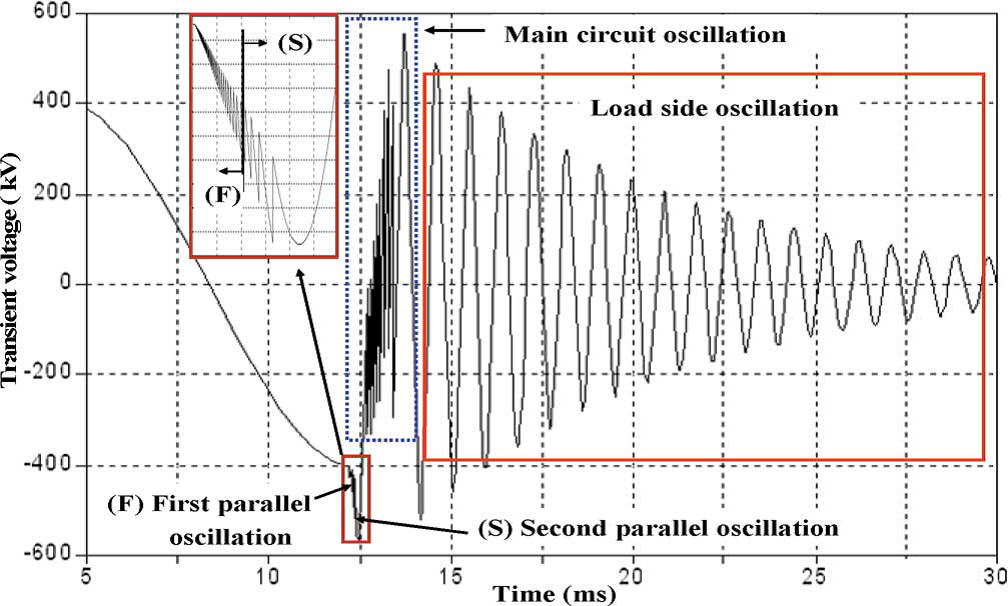
\includegraphics[width=\textwidth]{Oscillationmodesinreactorcircuit}
\caption[Oscillation Modes in Reactor Circuit]{Oscillation modes in reactor circuit \cite{chang2007modeling}}
\label{fig:Oscillation modes in reactor circuit}
\end{figure}

Circuit breaker interrupter failure is reported due to restrike which punctured right through the nozzle between the moving main contact and the fixed arcing contact of the interrupter \cite{lopez2007analysis}.

\section{Time Definitions as per IEC}
The Standard IEC 62271-100 \cite{AlternatingCurrentCircuit} covers the standard operating procedures for ac circuit breakers used for indoor or outdoor operation at 50 Hz and 60 Hz on the system having voltages above 1000 V. The most frequently used time definitions are -

\begin{description}[style=nextline]

\item[opening time] opening time is the interval of time between the instant of energizing the opening release, and the instant when the arcing contacts have separated in all poles, the circuit-breaker being in the closed position

\item[arcing time] interval of time between the instant of the first initiation of an arc and the instant of final arc extinction in all poles

\item[break time] interval of time between the beginning of the opening time of a mechanical switching device and the end of the arcing time

\item[closing time] the circuit-breaker being in the open position, closing time is the interval of time between energizing the closing circuit and the instant when the contacts touch in all poles

\item[make time] the circuit-breaker being in the open position, make time is the interval of time between energizing the closing circuit and the instant when the current begins to flow in the first pole

\item[pre-arcing time] during a closing operation, pre-arcing time is the interval of time between the initiation of current flow in the first pole and the instant when the contacts touch in all poles for three-phase conditions and the instant when the contacts touch in the arcing pole for single-phase conditions

\item[close-open time] interval of time between the instant when the contacts touch in the first pole during a closing operation and the instant when the arcing contacts have separated in all poles during the subsequent opening operation
\end{description}

Figures \ref{fig:Time Definitions during Opening and Closing, As Per IEC} to \ref{Fig:Time Definitions during Close-Open Cycle for CB without Switching Resistors} show the time definitions during opening and closing and close-open cycle respectively.

\begin{figure}[!htbp]
\centering
\begin{minipage}{\textwidth}
\centering
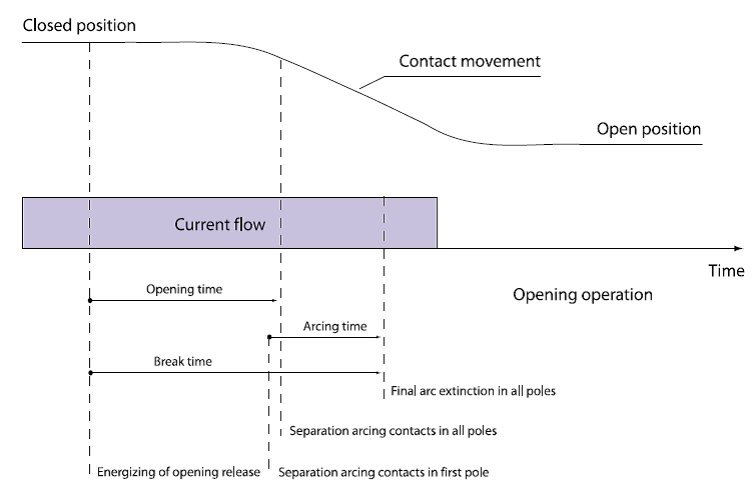
\includegraphics[width=\textwidth]{TimeDefinitionsduringOpeningandClosing1}
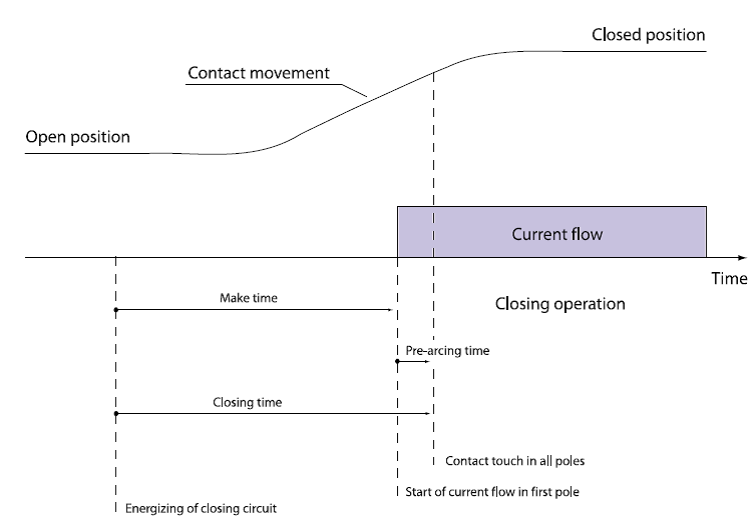
\includegraphics[width=\textwidth]{TimeDefinitionsduringOpeningandClosing2}
\caption{Time Definitions during Opening and Closing, As Per IEC}
\label{fig:Time Definitions during Opening and Closing, As Per IEC}
\end{minipage}
\end{figure}

\begin{sidewaysfigure}
   \centering 
   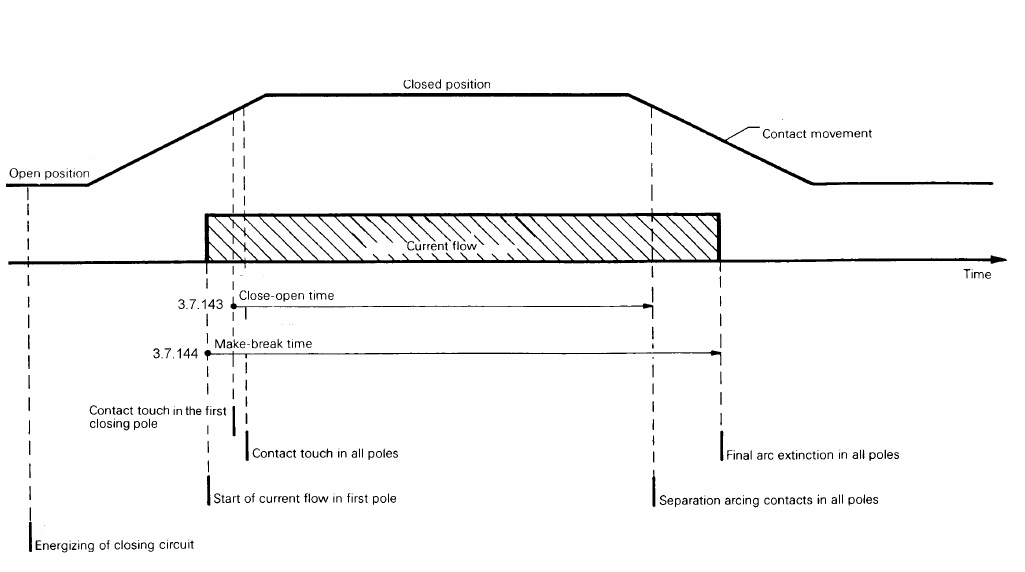
\includegraphics[width=\textwidth]{TimeDefinitionsduringCloseOpenCycleforCBwithout} 
   \caption{Time Definitions during Close-Open Cycle for CB without Switching Resistors}
   \label{Fig:Time Definitions during Close-Open Cycle for CB without Switching Resistors} 
\end{sidewaysfigure}

\subsection{Contact resistance measurement}

\subsubsection{Static contact resistance measurement (SCRM)}
Condition monitoring of CB through coil current signature, operational timings, tank gas pressure and the temperature is found \cite{dehghanian2014circuit, johal2008coil, natti2011assessing, guan2013assessing, biswas2015real, razi2015data }. However, coil current analysis does not give any information about contact condition. Generally, static contact resistance measurement is done to assess the condition of contacts. CB contacts are closed, and a DC current is passed through the contacts. IEC and ANSI recommend a value of 50A and 100A respectively. The voltage drop across the contacts is measured. The measured voltage drop, when divided by current, gives the resistance of main contacts. However, this method of resistance measurement evaluates the condition of main contacts only \cite{landry2006new}.

\subsubsection{Dynamic contact resistance measurement}
The condition of the arcing contacts is important from the point of short circuit current \setlength{\parskip}{1em} interruption capability of CB. It can be done by opening the CB interruption chamber. But this is time consuming and expensive due to high pressure SF\textsubscript{6} gas in the chamber. Also, reassembly of the unit may lead to new problems. DCRM is an indirect method of determining the condition of arcing contacts. It is quite similar to static contact resistance measurement with a difference that instead of a single value of resistance, a curve of resistance Vs time or distance is measured. Figure \ref{fig:Flow Chart of DCRM} gives the flow chart of DCRM. Close- open command is given to the CB and 100A DC current is injected. The instantaneous value of voltage and current is measured when CB opens. Resistance is calculated at each point. A curve of resistance Vs time is called as DCRM signature. DCRM signature along with the contact travel can be used to measure the main contact wipe, arcing contact wipe, average main contact and arcing contact resistance.

DCRMs during closing operations are not useful as the sudden change from infinity to the arcing contact resistance is difficult to measure. Also, undesired noise gets generated at the arcing contact touch \cite{landry2008complete}. Several spikes are observed in the DCRM curve due to partial contact separation for the CBs operated with a high speed of contact movement \cite{salamanca1993preventive, tyagi2001condition, ohlen1995dynamic}.

\setlength{\parskip}{0em}
\begin{figure}[!htbp]
\centering
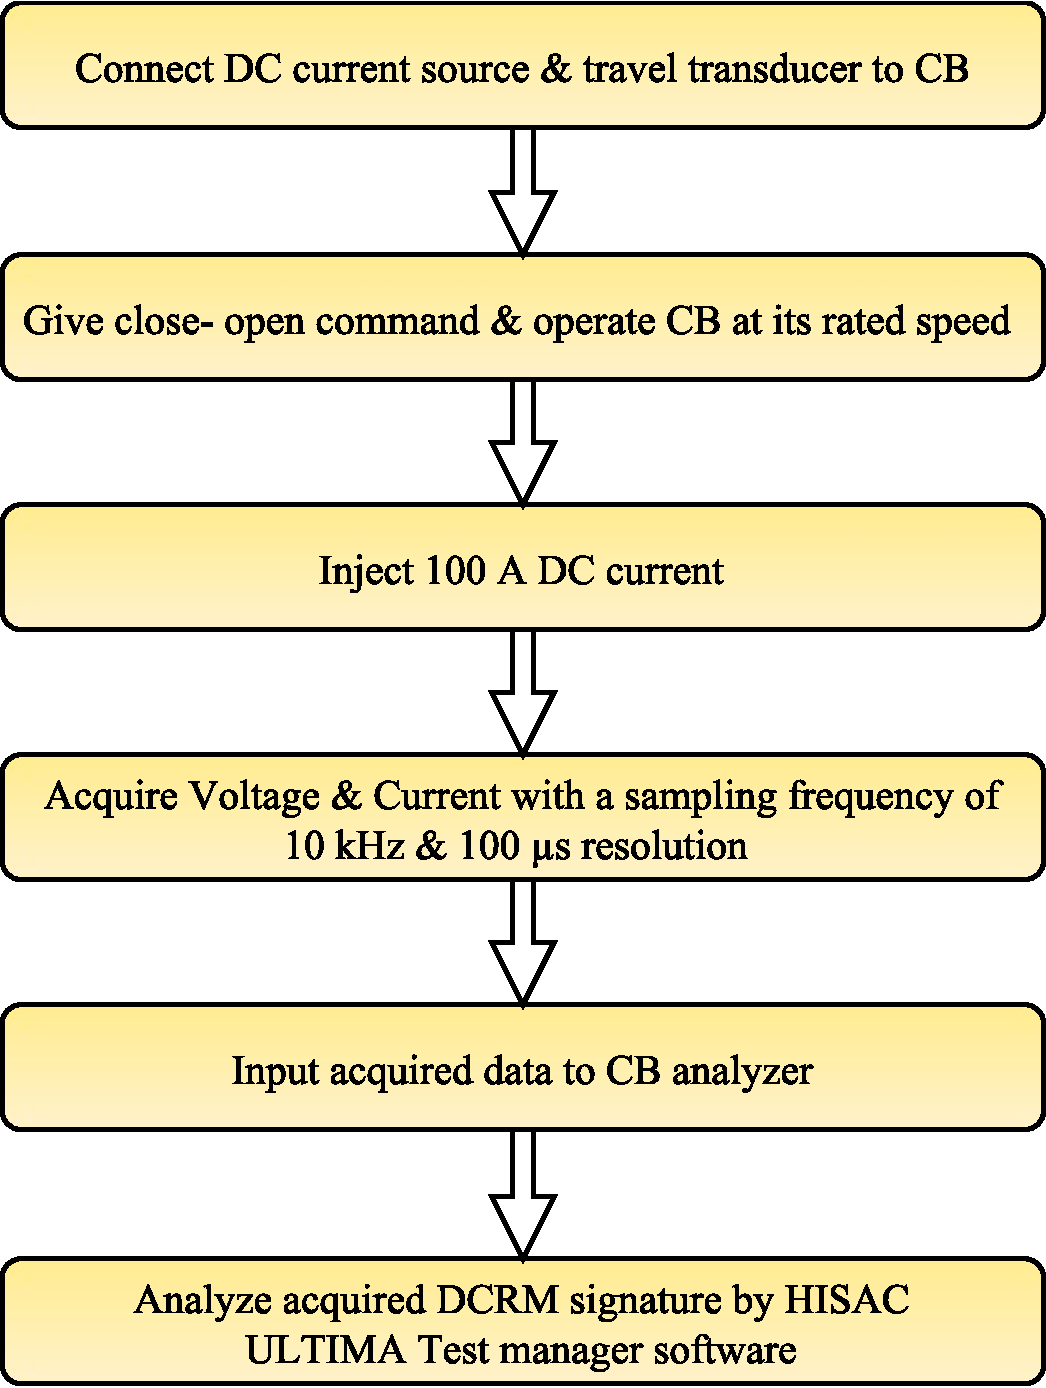
\includegraphics[width=\textwidth]{FlowChartofDCRM}
\caption{Flow Chart of DCRM}
\label{fig:Flow Chart of DCRM}
\end{figure}

\setlength{\parskip}{1em}
\textbf{Measurement at low speed}\\
M. Landry \textit{et al}. \cite{landry2006new} observed that the DCRM curves at rated speed are not comparable. The identification of main contact part was difficult. High contact speed was the reason anticipated for partial contact part. DCRMs at low speed were found identical. It was observed that the DCRM curves were smooth and the main contact parting was easy to identify. However, for some breaker mechanism, it is time-consuming to do the adjustments of a mechanism for low-speed operation. The CBs in the field are operated at rated speed. Hence the operation at low speed may not give the correct information of contacts.

\textbf{DCRM in the presence of metallic fluorides}\\
Due to arcing metallic fluorides are formed which get deposited on the CB contacts in the form of nonconductive dust powder. The effects of metallic fluorides on contact resistance have been dealt in \cite{tyagi2001condition}. High contact resistance was observed for the CB used for capacitor bank switching and which has performed a large number of operations. However, the deposition of metallic fluorides did not affect the short circuit capacity of CB. If the scraping or wiping action in the CB contact is not proper, then the high contact resistance will appear \cite{landry2006new}. Conventional equipment was used to perform the static contact resistance measurement at 100 A DC current. A high value of the contact resistance of the order of 4500-6000 $\mu \Omega$ was measured which could be interpreted as defective contacts. Michel Landry \textit{et al.} developed a method to determine the reason for high resistance which does not require the opening of CB interrupting chamber. Three current sources were connected in parallel to deliver 2800 A DC current. For carrying this high current from source to the breaker, six 4/0 copper cables were used. A measuring shunt of 51.32 $\Omega$ along with data acquisition system was used for recording the signals. Breaker contacts were kept in closed condition, and contacts were heated for different intervals in order to vaporize the metallic fluorides that were deposited on the CB contacts. DCRM were recorded for each phase at different currents. From this experimentation Michel Landry \textit{et al}. observed that heating of contacts for 15 minutes at 2800 A current reduced the arcing contact resistance to the acceptable level \cite{landry2008complete}.

\textbf{Measurement at low speed}\\
The conventional DCRM system needs heavy and long cables to connect the current source to the breaker. Ultra capacitors as a current source are discussed \cite{stanisic2010new}. The ultra capacitors along with constant charger are light weight as compared to batteries and are capable of generating few hundred amperes. A low resistance meter based on a large value of capacitor with a very small value of internal resistance, charger for the capacitor and control along with measurement circuitry for 250 A DC current was developed. The developed low resistance meter can be used for static as well as dynamic resistance measurements.

A DCRM system was developed using a stationary battery of 12V/220Ah  \cite{de2014characterization}. DCRM parameters that are useful in contact diagnosis are discussed.

A power grid experience of DCRM of CBs from PGCIL is shared \cite{sodha2012condition}. DCRM signatures of CBs from field with problems in contacts are described.

Erosion of arcing contact takes place during every operation of CB depending on the breaking current. The erosion of arcing contacts leads to the time difference between contact separations in successive operation. The contacts need the overhaul when the overlap time falls below a defined minimum value \cite{DynamicResistanceMeasurement}. 

On line monitoring of contact electrical erosion of CBs based on the theory of accumulative effect and the statistical average is developed \cite{fujie1998diagnosis}. 

High frequency DC/DC converter as a power source for generating high DC current and measuring the dynamic contact resistance of the CB is presented \cite{engineerdynamic}. 

Principal component analysis is used to get the information from dynamic resistance signal \cite{khoddam2016electrical}. 

Scoring and weighting techniques and health index are applied to identify the healthy, needs maintenance and risky condition of CB \cite{khoddam2016performance}.

Design and development process of control, acquisition, and analysis of the DCRM results for high voltage circuit breaker is presented \cite{obarvcanin2015design}.

Use of Arduino platform in measuring and processing the dynamic contact resistance curve is described \cite{de2014system}. However, it has the limitation of the sampling rate.

Testing of 400 kV CB in high induction environment is presented \cite{alibavsic2016new}. To overcome the induction voltage in recorded signal, grounding on both sides of HVCB is suggested.

All the work described in above papers focus on the measurement process of dynamic contact resistance. Methodology to detect the contact failure through DCRM is not discussed in the literature. Since the interrupter is sealed, it is not feasible to detect the contact condition. Intentional failure and then correlating the DCRM signature is not possible. 
\setlength{\parskip}{0em}

\section{Research Gap}
\setlength{\parskip}{1em}
Literature survey reveals that condition based maintenance has been the most efficient maintenance strategy. Lot of work has been done on the coil current analysis. Coil current signature can be acquired during the switching operation, and various approaches are available to determine the real time health of control circuit. Another crucial part of the circuit breakers is the main and arcing contacts.

It is observed that papers on Dynamic Contact Resistance Measurement focus on the measurement process of dynamic contact resistance. Methodology to detect the contact failure through DCRM is not discussed in the literature. Since the interrupter is sealed, it is not feasible to detect the contact condition. Intentional failure and then correlating the DCRM signature is not possible. 

The Dynamic Contact Resistance Measurement was developed around 20 years ago to assess the condition of arcing contacts without dismantling the breaker, and in India, the utility companies are using this test for condition monitoring from last ten years.

Arc formation and the TRV at the arc interruption of every CB connected to the same system configuration will be different. This is due to design aspect of CB. Hence every CB has a unique signature. Knowledge of CB design such as types of contacts, mechanism, the principle used in arc extinction, \textit{etc}. is necessary. Hence the signatures obtained from Dynamic Contact Resistance Measurement (DCRM) are difficult to interpret and may lead to wrong decisions about the condition of contacts. Signature analysis of circuit breaker for dynamic resistance measurement is developing. It is an emerging area for research.
\setlength{\parskip}{0em}